\subsubsection{\stid{3.01} xSDK} 
\paragraph{Overview} The xSDK project is creating a value-added aggregation of DOE math and scientific libraries through the xSDK~\cite{xsdk:homepage}, which increases the combined usability, standardization, and interoperability of these libraries as needed by ECP. The project focuses on community development and a commitment to combined success via quality improvement policies, better build infrastructure, and the ability to use diverse, independently developed xSDK libraries in combination to solve large-scale multiphysics and multiscale problems.  We are extending xSDK package community policies and developing interoperability layers among numerical libraries in order to improve code quality, access, usability, interoperability, and sustainability. Focus areas are (1) coordinated use of on-node resources, (2) integrated execution (control inversion and adaptive execution strategies), and (3) coordinated and sustainable documentation, testing, packaging, and deployment. %In FY20, the project also began to investigate and deploy multiprecision functionality in the ECP ST ecosystem to enable the use of low-precision hardware function units, reduce the pressure on memory and communication interfaces, and achieve improved performance.

xSDK is needed for ECP because it enables applications such as ExaAM and ExaWind to seamlessly leverage the entire scientific libraries ecosystem.  For example, ExaWind has extremely challenging linear solver scaling problems.  xSDK provides access to all scalable linear solvers with minimal changes.  xSDK is also an essential element of the product release process for ECP ST.  xSDK provides an aggregate build and install capability for all ECP math libraries that supports hierarchical, modular installation of ECP software.  Finally, xSDK provides a forum for collaborative math library development, helping independent teams to accelerate adoption of best practices, enabling interoperability of independently developed libraries and improving developer productivity and sustainability of the ECP ST software products.

\paragraph{Key Challenges}
The complexity of application codes is steadily increasing due to more sophisticated scientific models.  While some application areas will use Exascale platforms for higher fidelity, many are using the extra computing capability for increased coupling of scales and physics.  Without coordination, this situation  leads to difficulties when building application codes that use 8 or 10 different libraries, which in turn might require additional libraries or even different versions of the same libraries.

The xSDK represents a different approach to coordinating library development and deployment.  Prior to the xSDK, scientific software packages were cohesive with a single team effort, but not across these efforts. The xSDK goes a step further by developing community policies followed by each independent library included in the xSDK.  This policy-driven, coordinated approach enables independent development that still results in compatible and composable capabilities.

\paragraph{Solution Strategy}

The xSDK effort has two primary thrusts:
\begin{enumerate}
	\item \textbf{Increased interoperability:} xSDK packages can be built with a single Spack package target.  Furthermore, services from one package are accessible to another package.
	\item \textbf{Increased use of common best practices:}  The xSDK has a collection of community policies that set expectations for a package, from best design practices to common look-and-feel.
\end{enumerate}

xSDK interoperability efforts began first with eliminating incompatibilities that prohibited correct compilation and integration of the independently developed libraries.  These issues include being able to use a common version of a library by another library.  The second, and ongoing phase is increased use of one package's capabilities from another. xSDK community package policies~\cite{xsdk-policies:homepage,xsdk-policies:github} are a set of minimum requirements (including topics of configuring, installing, testing, MPI usage, portability, contact and version information, open source licensing, namespacing, and repository access) that a software package must satisfy in order to be considered xSDK compatible. The designation of xSDK compatibility informs potential users that a package can be easily used with others and makes configuration and installation of xSDK software and other HPC packages as efficient as possible on common platforms, including standard Linux distributions and Mac OS X, as well as on target machines currently available at DOE computing facilities (ALCF, NERSC, and OLCF) and eventually on new Exascale platforms.
Community policies for the xSDK promote long-term sustainability and interoperability among packages, as a foundation for supporting complex multiphysics and multiscale ECP applications. In addition, because new xSDK packages will follow the same standard, installation software and package managers (for example, Spack~\cite{gamblin+:sc15}) can easily be extended to install many packages automatically.

For the adaptive execution effort, the team is working toward GPTune, a Gaussian process tuner, to help math library users find the optimal parameter settings for the libraries to achieve high performance for their applications. In addition, an interface will be created to also give access to alternate autotuners.

Another effort in the project is the development of a software quality toolkit that automates analyses and activities related to code testing, documentation and use. The goal is to facilitate the use of both general-purpose and custom code analysis tools to improve the quality of the xSDK libraries, and, more broadly, software within the high-performance applications community.

\paragraph{Recent Progress}

The xSDK team released xSDK 0.6.0 with two new xSDK libraries heFFTe and SLATE and is preparing xSDK 0.7.0 with planned addition of ArborX.
Figure~\ref{fig:xsdk-schematic} illustrates the dependency graph of Spack-enabled interoperabilities of xSDK libraries in version 0.6.0 and the growth of the xSDK over the years .
\begin{figure}[htb]
	\centering
	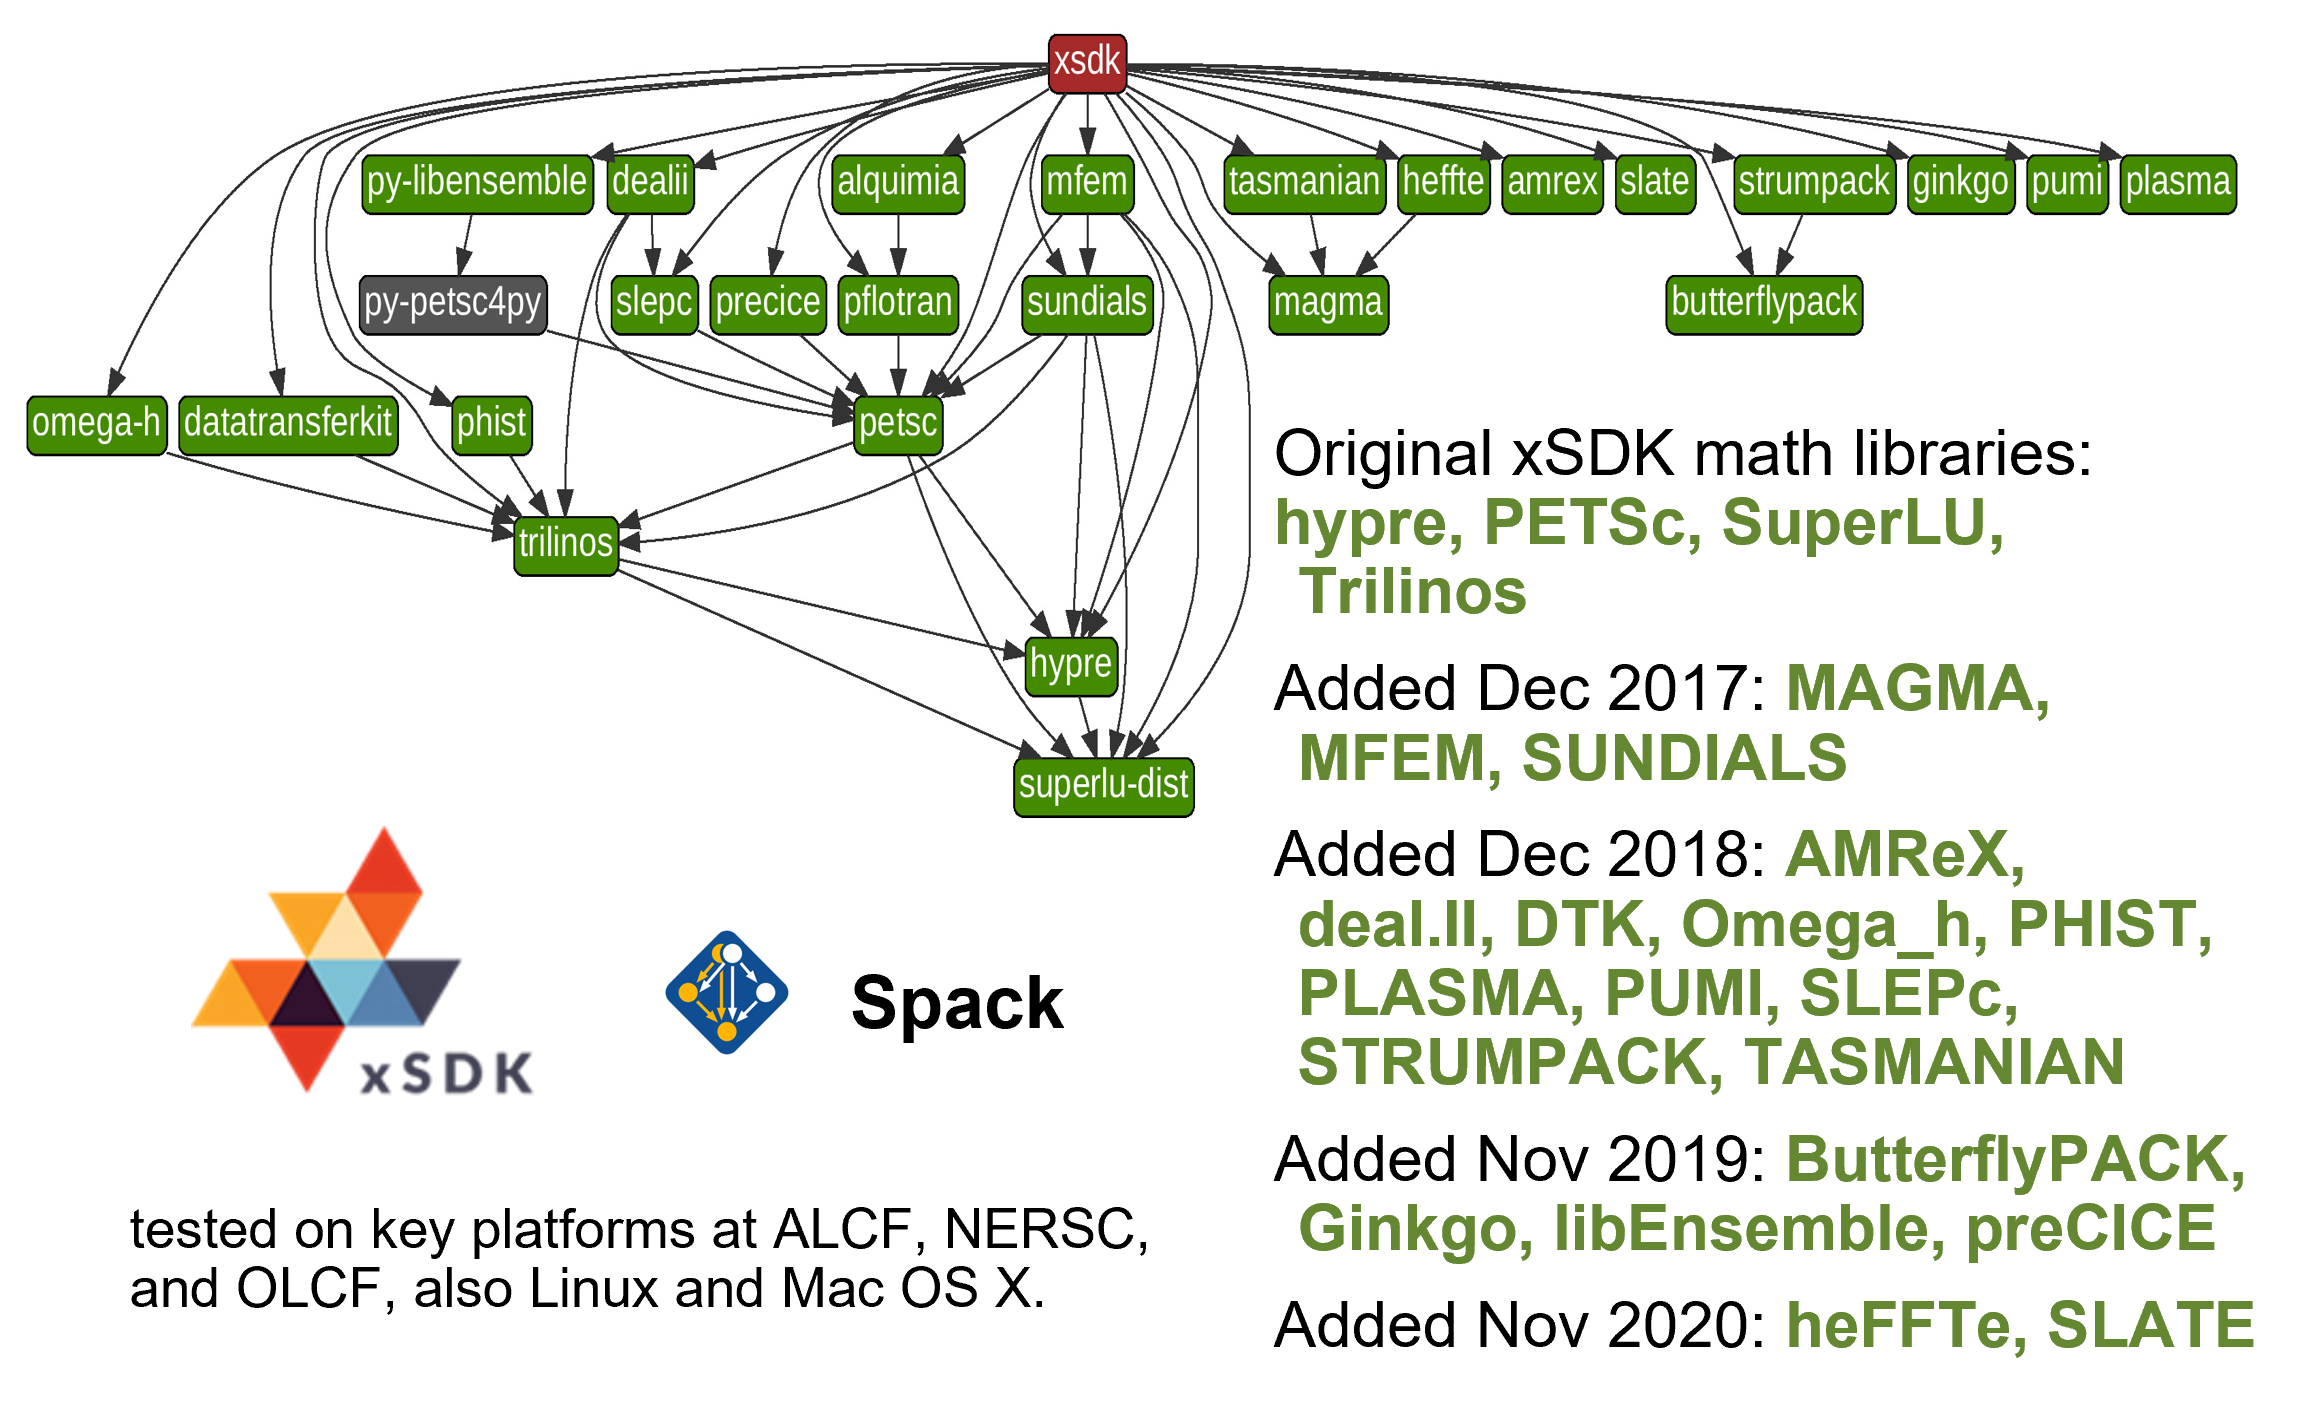
\includegraphics[width=4.2in]{projects/2.3.3-MathLibs/2.3.3.01-xSDK/xsdk-0.6.0.png}
	\caption{\label{fig:xsdk-schematic} Dependency graph of xSDK packages with Spack-enabled  interoperabilities represented in xSDK 0.6.0. A$\rightarrow$B indicates A uses B}
\end{figure}
The team also looked for ways to increase interoperability within the xSDK. To achieve this goal, package developers were surveyed for opportunities to increase interoperabilites and a report was provided summarizing survey results and new and planned interoperability capabilities between xSDK members. Version 0.2.0 of the xsdk-examples code suite was released with updated and expanded examples to demonstrate xSDK library interoperabilities, including some CUDA-enabled examples.

Version 2.0 of the GPTune auto-tuning software for parameter optimization of HPC codes \cite{gptune:homepage} was released. In this new release, the team finished the workflow design, with history database, shared repository and web interface for crowd-tuning. and developed the multi-fidelity GPTuneBand, combining LCM multitask learning and multi-armed bandit. The  GPTuneBand tuning algorithm was applied to the electromagnetic equations solvers in the finite element xSDK library MFEM, and achieved almost 2x speedup compared to the default parameter settings. 

The first version, v. 1.0.0, of a code quality toolkit, which contains open-source static and dynamic code analysis tools for C and C++, was released and applied to the xSDK libraries PETSc, Slepc, SUPERLU and hypre. Example codes are provided in the xsdk-code-quality repository \cite{xsdk-code-quality}.

\paragraph{Next Steps}

Our next efforts include 
\begin{itemize}
    \item development of a plan to improve xSDK testing with view towards sustainability,
    \item updating and enhancing the xsdk-examples test suite,
    \item implementation of the xSDK testing plan,
   \item a new xSDK release with additional libraries and build options for GPUs, including software, documentation and user engagement materials.
\end{itemize}

\newpage

